\documentclass[12pt, letterpaper]{article}
\usepackage{graphicx}
\graphicspath{{images/}}

\title{CCE5225 - Assignment 1 \\
\large MiniBooNE particle identification \\ signal/background classification}
\author{Sultan Dayani}
\date{December 2022}
\begin{document}
\maketitle
\pagebreak

\textgreater{Comment on whether the performance changes significantly amongst different hyperparameter values for each model.}
\textgreater{Report the time required for training, the set of hyperparameters which were tested, and the final per-class accuracies achieved on the unseen test set (in the form of a confusion matrix).}
\textgreater{Comment on the performance of each model, and provide an explanation as to why you believe the highest performing model gave the best results.}

# Vanilla Neural Network
Except for the stated parameters all others are the default from scikit-learn, e.g. solver='adam', activation='relu', etc.
Params: 'hidden_layer_sizes': [(10,), (20,), (30,), (40,), (50,)]
\begin{tabular}{|c c c|}
\hline
HL Size & Mean Fit Time & Mean Score \\ [0.5ex] 
\hline
(10,) & 99.88s & 0.927113 \\
\hline
(20,) & 100.26s & 0.931188 \\
\hline
(30,) & 74.61s & 0.933052 \\
\hline
(40,) & 376.35s & 0.935090 \\
\hline
(50,) & 163.39s & 0.933744 \\ 
\hline
\end{tabular}
The best performing model was the neural network with 40 neurons.
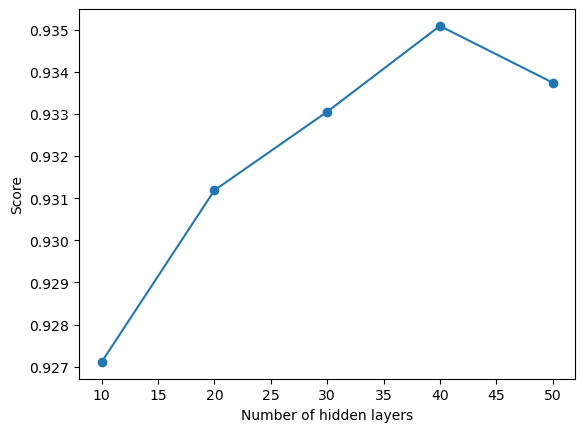
\includegraphics[width=0.6\textwidth]{1hiddenlayer_scores.png}

# Increasing the number of hidden layers
Choosing 30 for the size of neurons per hidden layer as it is the best performing size from the previous models.
Params: 'hidden_layer_sizes': [(40,), (40,40), (40,40,40), (40,40,40,40)],
HiddenLayerSize: (40,) | 75.29s | test-score: 0.935311
HiddenLayerSize: (40, 40) | 86.75s | test-score: 0.936723
HiddenLayerSize: (40, 40, 40) | 163.92s | test-score: 0.934984
HiddenLayerSize: (40, 40, 40, 40) | 249.26s | test-score: 0.932158

Using (40,40) and varying the activation function: \\
activation:  'relu' | 86.75s | test-score: 0.936723 \\ 
activation: 'logistic' | 168.04s | test-score: 0.930813 \\ 
activation: 'tanh' | 164.20s | test-score: 0.937665 \\ 
activation: 'identity' | 41.14s | test-score: 0.893321 \\ 
The activation function 'tanh' gave the best results but took double the time as 'relu'.

Considering the time to train the model, a double hidden layer with 30 neurons each, using the relu activation function is a good performing one.
hidden layer: (30,30), activation: 'relu' results in 101.86s build time and 0.939376 test score.

Comment:
The number of hidden layers helps a neural network to learn complex relationships, however too many hidden layers lead to overfitting which reduces performance.
It seems like two hidden layers with 30 neurons lead to a model that understands the relationship of the features well.
The activation functions lie close to each other, I believe the identity functions is the worst performing one as it is a linear function and the data is not linearly separable.

#SVM
Except for the stated hyperparameters all others are the default from scikit-learn, e.g. kernel='rbf', etc.
varying C on rbf:
C: 0.1 | 331.12s | test-score: 0.877185 \\
C: 1 | 160.40s | test-score: 0.891601 \\
C: 10 | 148.25s | test-score: 0.906661 \\
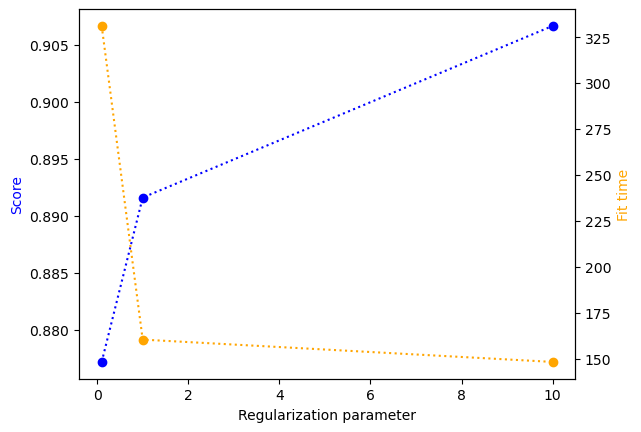
\includegraphics[width=0.6\textwidth]{svm_c_compiled.png}
The best performing model was the SVM with C=10.

varying kernel:
kernel: 'rbf' | 148.25s | test-score: 0.906661
kernel: 'linear' | 463.95s | test-score: 0.904653
kernel: 'poly' | 274.41s | test-score: 0.832592
kernel: 'sigmoid' | 393.91s | test-score: 0.728335

The best parameters are: {'C': 10, 'kernel': 'rbf'}

Comment:
Regularization encourages the model to find a balance between complexity and accuracy which lead to a better performing model.
I assume in this example rbf lead to the best results because it does a better job capturing the non-linear relationship between the features and the target.
And also because 'rbf' is tuned by a single hyperparameter and I did not tune the other models hyperparameters.

# Random Forest
Except for the stated hyperparameters all others are the default from scikit-learn, e.g. criterion='gini', etc.
N_estimators: 50 | 36.39s | test-score: 0.933821
N_estimators: 100 | 74.94s | test-score: 0.934926
N_estimators: 200 | 150.16s | test-score: 0.935503
No significant change in performance with the number of estimators.

For n_estimators = 50
max_depth: 5 | 11.74s | test-score: 0.893965
max_depth: 10 | 20.93s | test-score: 0.924643
max_depth: 15 | 29.69s | test-score: 0.932408
max_depth: 20 | 34.94s | test-score: 0.933984
max_depth: 25 | 36.65s | test-score: 0.933110
max_depth: 30 | 37.28s | test-score: 0.933225
20 is the best performing max_depth.

With n_estimators = 50 and max_depth = 20
min_samples_split: 2 | 35.98s | test-score: 0.933984
min_samples_split: 5 | 34.74s | test-score: 0.934388
min_samples_split: 10 | 34.60s | test-score: 0.933110


n_estimators: 50 | min_samples_split: 2 | max_depth: 10 | 22.33s | test-score: 0.924643 \\
n_estimators: 50 | min_samples_split: 2 | max_depth: 15 | 30.71s | test-score: 0.932408 \\
n_estimators: 50 | min_samples_split: 2 | max_depth: 20 | 36.04s | test-score: 0.933984 \\ \\
n_estimators: 50 | min_samples_split: 5 | max_depth: 10 | 22.69s | test-score: 0.924575 \\
n_estimators: 50 | min_samples_split: 5 | max_depth: 15 | 30.91s | test-score: 0.932860 \\
n_estimators: 50 | min_samples_split: 5 | max_depth: 20 | 35.91s | test-score: 0.934388 \\ \\
n_estimators: 50 | min_samples_split: 10 | max_depth: 10 | 22.65s | test-score: 0.924864 \\
n_estimators: 50 | min_samples_split: 10 | max_depth: 15 | 31.00s | test-score: 0.932552 \\
n_estimators: 50 | min_samples_split: 10 | max_depth: 20 | 35.57s | test-score: 0.933110 \\ \\ \\

n_estimators: 100 | min_samples_split: 2 | max_depth: 10 | 44.06s | test-score: 0.924883 \\
n_estimators: 100 | min_samples_split: 2 | max_depth: 15 | 62.45s | test-score: 0.933225 \\
n_estimators: 100 | min_samples_split: 2 | max_depth: 20 | 71.87s | test-score: 0.934695 \\ \\
n_estimators: 100 | min_samples_split: 5 | max_depth: 10 | 46.42s | test-score: 0.925114 \\
n_estimators: 100 | min_samples_split: 5 | max_depth: 15 | 62.23s | test-score: 0.933292 \\
n_estimators: 100 | min_samples_split: 5 | max_depth: 20 | 71.88s | test-score: 0.935205 \\ \\
n_estimators: 100 | min_samples_split: 10 | max_depth: 10 | 45.57s | test-score: 0.925162 \\
n_estimators: 100 | min_samples_split: 10 | max_depth: 15 | 64.83s | test-score: 0.933273 \\
n_estimators: 100 | min_samples_split: 10 | max_depth: 20 | 71.10s | test-score: 0.934484 \\ \\ \\

The best performing model is : {'max_depth': 20, 'min_samples_split': 5, 'n_estimators': 100} with a fit time of 71.88s and a test score of 0.935205.
/includegraphics[width=0.6\textwidth]{rf_n_estimators_compiled.png}
From the above graph, where max_depth is shown by hue and size is n_estimators, it is clear that the number of estimators and min sample size does not have a significant impact on the performance of the model. 
However the max_depth has a significant impact on the performance of the model. \\ 
Considering the time to train the model a random forest with n_estimators = 50, max_depth = 20 and min_samples_split = 5 is a good performing one with 35sec fit time and 0.934 accuracy.

Comment:
As seen from the data above the number of estimators or the min_samples_split does not have a significant impact on the performance of the model.
I believe max_depth has the biggest impact on the performance because it changes how complex of a pattern the model can learn.

\section{Conclusion}
Vanilla Neural Network confusion matrix:
Vanilla Neural Network hyperparameters: {'hidden_layer_sizes': (30, 30), 'activation': 'relu', 'max_iter': 500} Accuracy: 0.9393764656133472
\begin{matrix}
  17765 & 893\\
  684 & 6671
\end{matrix}
SVM confusion matrix:
SVM hyperparameters: {'C': 10} Accuracy: 0.908468842501826
\begin{matrix}
  17563 & 1095\\
  1286 & 6069
\end{matrix}
Random Forest confusion matrix:
Random Forest hyperparameters: {'max_depth': 20, 'min_samples_split': 5, 'n_estimators': 50} Accuracy: 0.9351862530273325
\begin{matrix}
17852 & 806\\
880 & 6475
\end{matrix}
Comment: I believe SVM is the worst performing model because it fails to capture the complexity and non-linear relationship of the features. It is also the slowest model to train. \\
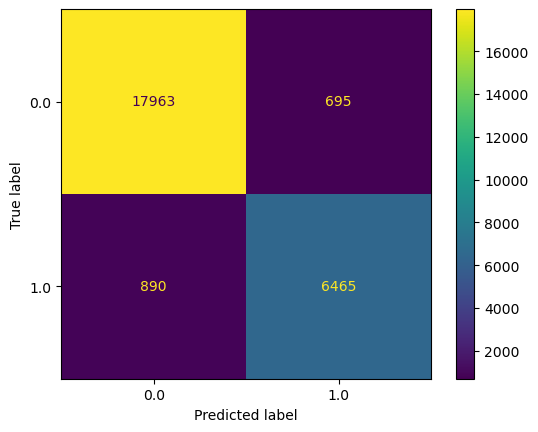
\includegraphics[width=0.3\textwidth]{vnn_confusion_matrix.png}
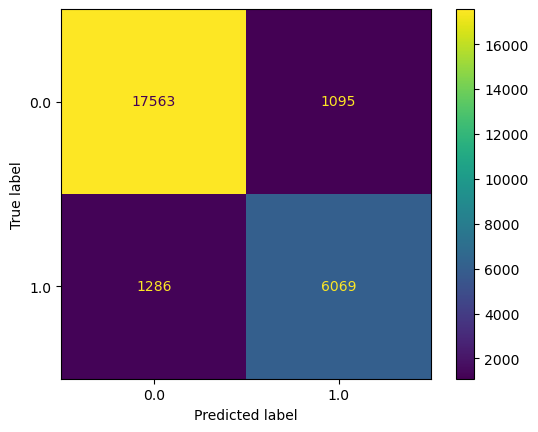
\includegraphics[width=0.3\textwidth]{svm_confusion_matrix.png}
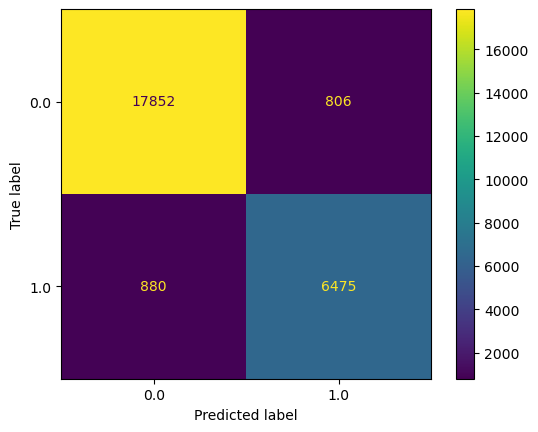
\includegraphics[width=0.3\textwidth]{rf_confusion_matrix.png}

\end{document}
